\chapter{Data Processing Using Pandas} \label{ch:pandas}

Many Python packages provide functions to handle structured data such as tables, series, and data frames. Among all these packages, \verb|pandas| is the all-time star that is very widely used by developers and data scientists. With \verb|pandas|, Python gains the ability to easily, flexibly and efficiently deal with data frames. The \verb|pandas| package is introduced in this section.

A large portion of this chapter, including codes and examples, are from online resources such as \textit{Data Analysis by Pandas and Python} on Udemy. My special thanks go to them.

The data frames used in the examples of this chapter may come from different public data resources. It is worth mentioning \textit{kaggle.com}, a place where tens of thousands of data sets, code examples, and notebooks are collected and shared. Some data frames used in the examples come from Kaggle.

Two Python packages, \verb|numpy| and \verb|pandas|, are almost certainly used in all the examples to be presented in this chapter. Import these packages as follows.
\begin{lstlisting}
import numpy as np
import pandas as pd
\end{lstlisting}
Unless otherwise mentioned, these packages are always assumed imported in this chapter. To display the packages version, use something like
\begin{lstlisting}
print("Numpy version: {}.".format(np.__version__))
print("Pandas version: {}".format(pd.__version__))
\end{lstlisting}

\section{Data Importing}

Pandas provide variety of ways to import data from different resources, including plain texts, CSV files, databases, etc. One of the most commonly seen data sources is CSV files. Importing data from CSV files is introduced here.

Pandas provide \verb|.read_csv()| function to import data from CSV files. Its basic usage is introduced below.
\begin{lstlisting}[language=python]
best_selling_games_df = pd.read_csv("best-selling-video-games.csv")
best_selling_games_df
\end{lstlisting}
which reads all the information in the CSV table into a data frame as shown by Fig. \ref{fig:dfexp}.
\begin{figure}[htbp]
	\centering
	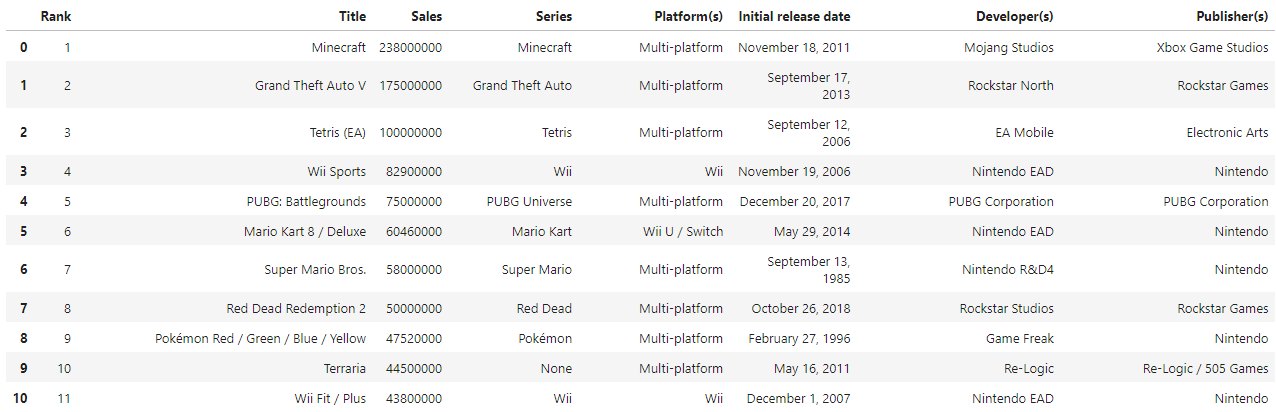
\includegraphics[width=\textwidth]{./chapters/ch-python/figures/df_example.png}
	\caption{The simplest data frame importing using pandas.}
	\label{fig:dfexp}
\end{figure}
It is possible to import only selected columns as follows.
\begin{lstlisting}[language=python]
best_selling_games_df = pd.read_csv("best-selling-video-games.csv", usecols = ["Title", "Sales", "Publisher(s)"])
best_selling_games_df
\end{lstlisting}

When no index column is specified, pandas will add an additional auto-incremental column and use it as the index column, as shown in Fig. \ref{fig:dfexp} by the most-left column. When a column index is specified, pandas will use that column as index column. An example is given below. The result is shown in Fig. \ref{fig:dfex2}.
\begin{lstlisting}[language=python]
best_selling_games_df = pd.read_csv("best-selling-video-games.csv", index_col = "Title", usecols = ["Title", "Sales", "Publisher(s)"])
best_selling_games_df
\end{lstlisting}
\begin{figure}[htbp]
	\centering
	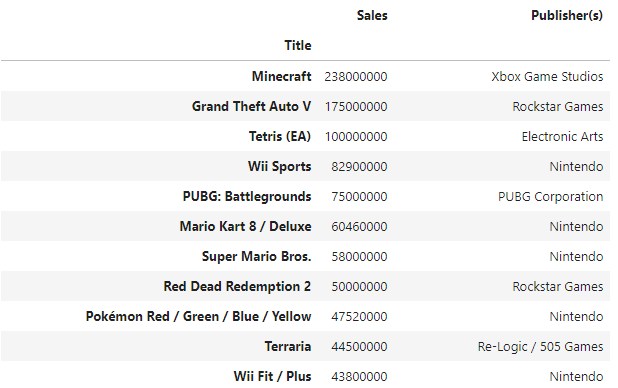
\includegraphics[width=0.5\textwidth]{./chapters/ch-python/figures/df_example2.png}
	\caption{Specifying index column and reading only selected columns using pandas.}
	\label{fig:dfex2}
\end{figure}

It is possible to read the full-size data frame into pandas first, then subsequently select only a few (or event only one) columns to form a new sub data frame. It is possible to take only one column from the data frame, and convert it into a series. Notice that a single-column data frame is different from a series from data type perspective. Examples are given below.
\begin{lstlisting}
# form sub data frame
best_selling_games_df = pd.read_csv("best-selling-video-games.csv")
sub_games_df = best_selling_games_df[["Title", "Sales", "Publisher(s)"]]
sub_games_df
# form single-column sub data frame
sub_games_df = best_selling_games_df[["Title"]]
sub_games_df
# convert single-column data frame to series
best_selling_games_titles = sub_games_df.squeeze('columns')
best_selling_games_titles
# get series from data frame directly
best_selling_games_df = pd.read_csv("best-selling-video-games.csv")
best_selling_games_titles = best_selling_games_df["Title"]
best_selling_games_titles
\end{lstlisting}

It is worth mentioning that when generating series from data frames, the index column of the data frame is inherited by the series. This introduces an important feature of pandas series: unlike Python array where it is just single-stream sequence of data, pandas series has a separate measure of index for each element in the series, essentially making it multi-stream of data. More are introduced in later sections.

\section{Series and Data Frame}

